\section{Негладкие начальные данные}
Для системы (1) на области $Q = [0; T] \times [0, 10]$ зададим две задачи со следующими начальными и граничными условиями:
\begin{equation}
	\begin{cases}
		$$
		\rho_0 (x) = 1, \ \ x < 4.5 \ \text{или} \  x > 5.5,
		\\
		\rho_0 (x) = 2, \ \ x \in [4.5; 5.5], 
		\\
		u_0 (x) \equiv 0, \ \ x \in [0; 10], 
		\\
		u (t, 0) = u (t, 10) = 0, \ \ t \in [0; T], 
		\\
		f \equiv 0.
		$$
	\end{cases}
\end{equation}

\begin{equation}
	\begin{cases}
		$$
		u_0 (x) = 0, \ \ x < 4.5 \ \text{или} \  x > 5.5,
		\\
		u_0 (x) = 1, \ \ x \in [4.5; 5.5], 
		\\
		\rho_0 (x) \equiv 1, \ \ x \in [0; 10], 
		\\
		u (t, 0) = u (t, 10) = 0, \ \ t \in [0; T],
		\\
		f \equiv 0.
		$$
	\end{cases}
\end{equation}

\subsection{Результаты}
Ниже приведены таблицы содержащие времена стабилизации $T_{st}$ решений первой системы и величин $|| (H^{n_{st}}, V^{n_{st}}) - (\tilde{H}, \tilde{V})||_{C_h}$ при различных входных параметрах (строки таблицы) на разных временных слоях (столбцы таблицы). Так же приведены таблицы, содержащие величины 
\begin{equation*}
	\displaystyle \Delta_m (n) = \frac{\sum\limits_{m \in \bar{\omega}_h} H^n_m - \sum\limits_{m \in \bar{\omega}_h} H^0_m}{\sum\limits_{m \in \bar{\omega}_h} H^0_m}
\end{equation*}
на разных временных слоях (столбцы таблицы) при различных входных параметрах (строки таблицы).
\subsubsection{Таблицы для первой системы}
1. $C_{\rho} = 1, \ \mu = 0.1$
\begin{center}
	\begin{tabular}{ |c|c|c|c|c|c| } 
		\hline
		$\tau$, h & $n_{st}/ 4$ & $n_{st}/ 2$ & $3n_{st}/ 4$ & $n_{st}$ & $T_{st}$ \\ 
		\hline
		1e-01, 1e-01 & 9.516e-02 & 5.305e-02 & 1.740e-02 & 9.854e-03 & 194.1\\ 
		\hline
		1e-01, 1e-02 & 4.323e-02 & 2.218e-02 & 1.528e-02 & 9.846e-03 & 971.4\\ 
		\hline
		1e-02, 1e-01 & 8.427e-02 & 4.164e-02 & 2.134e-02 & 9.980e-03 & 118.33\\ 
		\hline
		1e-02, 1e-02 & 9.044e-02 & 5.022e-02 & 1.988e-02 & 9.967e-03 & 147.8\\ 
		\hline
	\end{tabular}
\end{center}

\begin{center}
	\begin{tabular}{ |c|c|c|c|c| } 
		\hline
		$\tau$, h & $\Delta_m (n_{st}/ 4)$ & $\Delta_m (n_{st}/ 2)$ & $\Delta_m (3n_{st}/ 4)$ & $\Delta_m (n_{st})$ \\ 
		\hline
		1e-01, 1e-01 & 2.878e-01 & 3.276e-01 & 3.402e-01 & 3.460e-01 \\ 
		\hline
		1e-01, 1e-02 & 1.860e-01 & 1.942e-01 & 2.045e-01 & 2.139e-01 \\ 
		\hline
		1e-02, 1e-01 & 4.446e-02 & 5.677e-02 & 6.343e-02 & 6.723e-02 \\ 
		\hline
		1e-02, 1e-02 & 6.303e-03 & 8.453e-03 & 9.524e-03 & 1.005e-02 \\ 
		\hline
	\end{tabular}
\end{center}

2. $C_{\rho} = 1, \ \mu = 0.01$
\begin{center}
	\begin{tabular}{ |c|c|c|c|c|c| } 
		\hline
		$\tau$, h & $n_{st}/ 4$ & $n_{st}/ 2$ & $3n_{st}/ 4$ & $n_{st}$ & $T_{st}$ \\ 
		\hline
		1e-02, 1e-02 & 1.270e-02 & 3.405e-03 & 6.962e-03 & 9.916e-05 & 4514.51\\ 
		\hline
		1e-02, 1e-03 & 7.186e-02 & 6.282e-02 & 4.064e-02 & 2.497e-02 & 240.23\\ 
		\hline
		1e-03, 1e-01 & 5.705e-01 & 2.974e-01 & 3.087e-01 & 9.991e-05 & 567.562\\ 
		\hline
		1e-03, 1e-02 & 6.306e-02 & 2.327e-02 & 1.730e-02 & 9.997e-03 & 469.172\\ 
		\hline
	\end{tabular}
\end{center}

\begin{center}
	\begin{tabular}{ |c|c|c|c|c| } 
		\hline
		$\tau$, h & $\Delta_m (n_{st}/ 4)$ & $\Delta_m (n_{st}/ 2)$ & $\Delta_m (3n_{st}/ 4)$ & $\Delta_m (n_{st})$ \\ 
		\hline
		1e-02, 1e-02 & 4.048e-01 & 4.083e-01 & 4.152e-01 & 4.297e-01 \\ 
		\hline
		1e-02, 1e-03 & 1.825e-01 & 1.980e-01 & 2.125e-01 & 2.235e-01 \\ 
		\hline
		1e-03, 1e-01 & 4.437e-01 & 7.689e-01 & 7.875e-01 & 8.278e-01 \\ 
		\hline
		1e-03, 1e-02 & 4.534e-02 & 5.513e-02 & 5.919e-02 & 6.138e-02 \\ 
		\hline
	\end{tabular}
\end{center}

3. $C_{\rho} = 1, \ \mu = 0.001$
\begin{center}
	\begin{tabular}{ |c|c|c|c|c|c| } 
		\hline
		$\tau$, h & $n_{st}/ 4$ & $n_{st}/ 2$ & $3n_{st}/ 4$ & $n_{st}$ & $T_{st}$ \\ 
		\hline
		1e-03, 1e-03 & 2.703e-01 & 3.388e-01 & 1.268e-01 & 9.923e-02 & 8.055\\ 
		\hline
		1e-03, 1e-02 & 3.207e-02 & 3.094e-02 & 2.640e-02 & 9.994e-03 & 287.015\\ 
		\hline
		1e-04, 1e-02 & 5.505e-01 & 9.773e-02 & 7.496e-02 & 5.000e-02 & 20.9462\\ 
		\hline
		5e-04, 1e-02 & 8.598e-02 & 2.833e-02 & 3.081e-02 & 9.995e-03 & 71.401\\ 
		\hline
	\end{tabular}
\end{center}

\begin{center}
	\begin{tabular}{ |c|c|c|c|c| } 
		\hline
		$\tau$, h & $\Delta_m (n_{st}/ 4)$ & $\Delta_m (n_{st}/ 2)$ & $\Delta_m (3n_{st}/ 4)$ & $\Delta_m (n_{st})$ \\ 
		\hline
		1e-03, 1e-03 & 1.988e-01 & 3.042e-01 & 3.624e-01 & 3.782e-01 \\ 
		\hline
		1e-03, 1e-02 & -8.388e-01 & -8.408e-01 & -8.420e-01 & -8.429e-01 \\ 
		\hline
		1e-04, 1e-02 & -6.097e-01 & -7.958e-01 & -8.044e-01 & -8.075e-01 \\ 
		\hline
		5e-04, 1e-02 & -8.174e-01 & -8.239e-01 & -8.258e-01 & -8.266e-01 \\ 
		\hline
	\end{tabular}
\end{center}

4. $C_{\rho} = 10, \ \mu = 0.1$
\begin{center}
	\begin{tabular}{ |c|c|c|c|c|c| } 
		\hline
		$\tau$, h & $n_{st}/ 4$ & $n_{st}/ 2$ & $3n_{st}/ 4$ & $n_{st}$ & $T_{st}$ \\ 
		\hline
		1e-02, 1e-02 & 3.055e-02 & 8.490e-03 & 3.398e-03 & 9.931e-04 & 1535.55\\ 
		\hline
		1e-03, 1e-02 & 3.397e-02 & 2.408e-02 & 5.634e-03 & 9.971e-04 & 250.899\\ 
		\hline
		1e-02, 1e-01 & 8.759e-02 & 8.567e-03 & 9.062e-04 & 1.799e-04 & 189.17\\ 
		\hline
		1e-03, 1e-02 & 3.418e-02 & 4.385e-03 & 1.459e-03 & 4.996e-04 & 120.736\\ 
		\hline
	\end{tabular}
\end{center}

\begin{center}
	\begin{tabular}{ |c|c|c|c|c| } 
		\hline
		$\tau$, h & $\Delta_m (n_{st}/ 4)$ & $\Delta_m (n_{st}/ 2)$ & $\Delta_m (3n_{st}/ 4)$ & $\Delta_m (n_{st})$ \\ 
		\hline
		1e-02, 1e-02 & -2.894e-01 & -3.299e-01 & -3.448e-01 & -3.509e-01 \\ 
		\hline
		1e-03, 1e-02 & -2.571e-02 & -2.826e-02 & -2.901e-02 & -2.927e-02 \\ 
		\hline
		1e-02, 1e-01 & -5.950e-01 & -6.071e-01 & -6.155e-01 & -6.159e-01 \\ 
		\hline
		1e-03, 1e-01 & -4.153e-01 & -4.217e-01 & -4.227e-01 & -4.233e-01 \\ 
		\hline
	\end{tabular}
\end{center}

5. $C_{\rho} = 10, \ \mu = 0.01$
\begin{center}
	\begin{tabular}{ |c|c|c|c|c|c| } 
		\hline
		$\tau$, h & $n_{st}/ 4$ & $n_{st}/ 2$ & $3n_{st}/ 4$ & $n_{st}$ & $T_{st}$ \\ 
		\hline
		1e-04, 1e-02 & 9.426e-02 & 5.507e-02 & 2.663e-02 & 9.998e-03 & 283.8961\\ 
		\hline
		1e-03, 1e-02 & 3.755e-02 & 3.327e-02 & 2.242e-02 & 9.986e-03 & 315.399\\ 
		\hline
		1e-03, 1e-03 & 1.902e-01 & 8.003e-02 & 7.652e-02 & 4.986e-02 & 51.174\\ 
		\hline
		1e-04, 1e-03 & 3.442e-01 & 1.964e-01 & 2.382e-01 & 1.000e-01 & 43.6666\\ 
		\hline
	\end{tabular}
\end{center}

\begin{center}
	\begin{tabular}{ |c|c|c|c|c| } 
		\hline
		$\tau$, h & $\Delta_m (n_{st}/ 4)$ & $\Delta_m (n_{st}/ 2)$ & $\Delta_m (3n_{st}/ 4)$ & $\Delta_m (n_{st})$ \\ 
		\hline
		1e-04, 1e-02 & -4.437e-01 & -4.533e-01 & -4.569e-01 & -4.585e-01 \\ 
		\hline
		1e-03, 1e-02 & -6.330e-01 & -6.358e-01 & -6.372e-01 & -6.379e-01 \\ 
		\hline
		1e-03, 1e-03 & -2.557e-01 & -2.769e-01 & -2.875e-01 & -2.948e-01 \\ 
		\hline
		1e-04, 1e-03 & -1.177e-02 & -1.660e-02 & -2.002e-02 & -2.274e-02 \\ 
		\hline
	\end{tabular}
\end{center}

6. $C_{\rho} = 10, \ \mu = 0.001$
\begin{center}
	\begin{tabular}{ |c|c|c|c|c|c| } 
		\hline
		$\tau$, h & $n_{st}/ 4$ & $n_{st}/ 2$ & $3n_{st}/ 4$ & $n_{st}$ & $T_{st}$ \\ 
		\hline
		1e-03, 1e-02 & 6.506e-02 & 3.475e-02 & 4.556e-02 & 9.995e-03 & 348.109\\ 
		\hline
		1e-04, 1e-03 & 3.077e-01 & 1.115e-01 & 8.026e-02 & 4.997e-02 & 17.661\\ 
		\hline
		5e-04, 1e-02 & 1.107e-01 & 7.850e-02 & 4.811e-02 & 9.989e-03 & 211.498\\ 
		\hline
		5e-04, 5e-03 & 1.992e-01 & 1.394e-01 & 9.121e-02 & 4.994e-02 & 56.98\\ 
		\hline
	\end{tabular}
\end{center}

\begin{center}
	\begin{tabular}{ |c|c|c|c|c| } 
		\hline
		$\tau$, h & $\Delta_m (n_{st}/ 4)$ & $\Delta_m (n_{st}/ 2)$ & $\Delta_m (3n_{st}/ 4)$ & $\Delta_m (n_{st})$ \\ 
		\hline
		1e-03, 1e-02 & -9.633e-01 & -9.636e-01 & -9.638e-01 & -9.638e-01 \\ 
		\hline
		1e-04, 1e-03 & -6.316e-01 & -6.351e-01 & -6.367e-01 & -6.379e-01 \\ 
		\hline
		5e-04, 1e-02 & -9.542e-01 & -9.546e-01 & -9.547e-01 & -9.548e-01 \\ 
		\hline
		5e-04, 5e-03 & -9.251e-01 & -9.262e-01 & -9.266e-01 & -9.268e-01 \\ 
		\hline
	\end{tabular}
\end{center}

7. $C_{\rho} = 100, \ \mu = 0.1$
\begin{center}
	\begin{tabular}{ |c|c|c|c|c|c| } 
		\hline
		$\tau$, h & $n_{st}/ 4$ & $n_{st}/ 2$ & $3n_{st}/ 4$ & $n_{st}$ & $T_{st}$ \\ 
		\hline
		1e-03, 1e-02 & 1.896e-02 & 8.329e-03 & 7.465e-03 & 9.973e-04 & 364.908\\ 
		\hline
		1e-04, 1e-02 & 2.207e-01 & 7.573e-02 & 2.956e-02 & 9.991e-03 & 87.9375\\ 
		\hline
		1e-03, 1e-03 & 1.558e-01 & 9.272e-02 & 7.836e-02 & 9.845e-03 & 235.576\\ 
		\hline
		1e-04, 5e-03 & 8.927e-01 & 4.448e-01 & 2.176e-01 & 1.000e-01 & 28.3531\\ 
		\hline
	\end{tabular}
\end{center}

\begin{center}
	\begin{tabular}{ |c|c|c|c|c| } 
		\hline
		$\tau$, h & $\Delta_m (n_{st}/ 4)$ & $\Delta_m (n_{st}/ 2)$ & $\Delta_m (3n_{st}/ 4)$ & $\Delta_m (n_{st})$ \\ 
		\hline
		1e-03, 1e-02 & -4.084e-01 & -4.208e-01 & -4.263e-01 & -4.286e-01 \\ 
		\hline
		1e-04, 1e-02 & -5.439e-02 & -6.094e-02 & -6.333e-02 & -6.455e-02 \\ 
		\hline
		1e-03, 1e-03 & -2.569e-01 & -2.844e-01 & -2.965e-01 & -3.081e-01 \\ 
		\hline
		1e-04, 5e-03 & -2.421e-02 & -3.201e-02 & -3.571e-02 & -3.769e-02 \\ 
		\hline
	\end{tabular}
\end{center}

8. $C_{\rho} = 100, \ \mu = 0.01$
\begin{center}
	\begin{tabular}{ |c|c|c|c|c|c| } 
		\hline
		$\tau$, h & $n_{st}/ 4$ & $n_{st}/ 2$ & $3n_{st}/ 4$ & $n_{st}$ & $T_{st}$ \\ 
		\hline
		1e-04, 1e-02 & 3.542e-01 & 2.700e-01 & 1.301e-01 & 4.998e-02 & 29.5694\\ 
		\hline
		1e-04, 1e-03 & 3.598e-01 & 1.984e-01 & 2.108e-01 & 9.997e-02 & 15.0497\\ 
		\hline
		1e-04, 5e-03 & 5.811e-01 & 3.914e-01 & 2.211e-01 & 9.983e-02 & 16.6602\\ 
		\hline
		1e-04, 1e-04 & 2.467e-01 & 1.543e-01 & 1.124e-01 & 9.994e-02 & 13.6379\\ 
		\hline
	\end{tabular}
\end{center}

\begin{center}
	\begin{tabular}{ |c|c|c|c|c| } 
		\hline
		$\tau$, h & $\Delta_m (n_{st}/ 4)$ & $\Delta_m (n_{st}/ 2)$ & $\Delta_m (3n_{st}/ 4)$ & $\Delta_m (n_{st})$ \\ 
		\hline
		1e-04, 1e-02 & -8.399e-01 & -8.415e-01 & -8.428e-01 & -8.431e-01 \\ 
		\hline
		1e-04, 1e-03 & -3.999e-01 & -4.064e-01 & -4.101e-01 & -4.125e-01 \\ 
		\hline
		1e-04, 5e-03 & -7.235e-01 & -7.280e-01 & -7.295e-01 & -7.302e-01 \\ 
		\hline
		1e-04, 1e-04 & -2.779e-01 & -3.081e-01 & -3.111e-01 & -3.158e-01 \\ 
		\hline
	\end{tabular}
\end{center}

9. $C_{\rho} = 100, \ \mu = 0.001$
\begin{center}
	\begin{tabular}{ |c|c|c|c|c|c| } 
		\hline
		$\tau$, h & $n_{st}/ 4$ & $n_{st}/ 2$ & $3n_{st}/ 4$ & $n_{st}$ & $T_{st}$ \\ 
		\hline
		1e-05, 1e-04 & 3.927e-01 & 1.930e-01 & 1.652e-01 & 9.997e-02 & 7.54607\\ 
		\hline
		1e-05, 5e-04 & 4.593e-01 & 3.039e-01 & 2.049e-01 & 1.000e-02 & 7.38283\\ 
		\hline
		1e-05, 1e-05 & 2.394e-01 & 2.103e-01 & 1.329e-01 & 9.977e-02 & 10.29393\\ 
		\hline
		1e-05, 5e-05 & 2.684e-01 & 2.111e-01 & 1.993e-01 & 9.991e-02 & 11.38456\\ 
		\hline
	\end{tabular}
\end{center}

\begin{center}
	\begin{tabular}{ |c|c|c|c|c| } 
		\hline
		$\tau$, h & $\Delta_m (n_{st}/ 4)$ & $\Delta_m (n_{st}/ 2)$ & $\Delta_m (3n_{st}/ 4)$ & $\Delta_m (n_{st})$ \\ 
		\hline
		1e-05, 1e-04 & -4.105e-01 & -4.162e-01 & -4.194e-01 & -4.210e-01 \\ 
		\hline
		1e-05, 5e-04 & -5.294e-01 & -5.322e-01 & -5.284e-01 & -5.099e-01 \\ 
		\hline
		1e-05, 1e-05 & -3.954e-01 & -2.495e-01 &-2.584e-01  & -2.335e-01 \\ 
		\hline
		1e-05, 5e-05 & -4.003e-01 & -3.489e-01 & -3.484e-01 & -4.471e-01 \\ 
		\hline
	\end{tabular}
\end{center}

10. $\gamma = 1.4, \ \mu = 0.1$
\begin{center}
	\begin{tabular}{ |c|c|c|c|c|c| } 
		\hline
		$\tau$, h & $n_{st}/ 4$ & $n_{st}/ 2$ & $3n_{st}/ 4$ & $n_{st}$ & $T_{st}$ \\ 
		\hline
		1e-01, 1e-01 & 1.628e-03 & 7.137e-05 & 3.208e-06 & 9.808e-08 & 1174.5\\ 
		\hline
		1e-02, 1e-01 & 4.478e-03 & 2.937e-04 & 1.696e-05 & 9.987e-07 & 723.81\\ 
		\hline
		1e-02, 1e-02 & 1.081e-03 & 1.155e-05 & 1.125e-07 & 9.990e-10 & 1215.69\\ 
		\hline
		1e-03, 1e-02 & 7.882e-02 & 4.349e-02 & 2.309e-02 & 9.997e-03 & 131.03\\ 
		\hline
	\end{tabular}
\end{center}

\begin{center}
	\begin{tabular}{ |c|c|c|c|c| } 
		\hline
		$\tau$, h & $\Delta_m (n_{st}/ 4)$ & $\Delta_m (n_{st}/ 2)$ & $\Delta_m (3n_{st}/ 4)$ & $\Delta_m (n_{st})$ \\ 
		\hline
		1e-01, 1e-01 & -4.803e-01 & -4.813e-01 & -4.813e-01 & -4.813e-01 \\ 
		\hline
		1e-02, 1e-01 & -8.755e-02 & -8.997e-02 & -9.012e-02 & -9.013e-02 \\ 
		\hline
		1e-02, 1e-02 & -1.349e-02 & -1.355e-02 & -1.355e-02 & -1.355e-02 \\ 
		\hline
		1e-03, 1e-02 & -7.285e-03 & -9.570e-03 & -1.058e-02 & -1.108e-02 \\ 
		\hline
	\end{tabular}
\end{center}

11. $\gamma = 1.4, \ \mu = 0.01$
\begin{center}
	\begin{tabular}{ |c|c|c|c|c|c| } 
		\hline
		$\tau$, h & $n_{st}/ 4$ & $n_{st}/ 2$ & $3n_{st}/ 4$ & $n_{st}$ & $T_{st}$ \\ 
		\hline
		1e-02, 1e-01 & 9.412e-04 & 1.772e-05 & 1.385e-07 & 9.990e-09 & 2065.51\\ 
		\hline
		1e-02, 1e-02 & 9.819e-03 & 4.873e-03 & 2.611e-03 & 9.998e-04 & 1455.74\\ 
		\hline
		1e-03, 1e-02 & 5.631e-02 & 2.713e-02 & 1.495e-02 & 9.999e-03 & 318.643\\ 
		\hline
		1e-02, 1e-03 & 6.862e-02 & 2.844e-02 & 1.597e-02 & 9.979e-03 & 254.46\\ 
		\hline
	\end{tabular}
\end{center}

\begin{center}
	\begin{tabular}{ |c|c|c|c|c| } 
		\hline
		$\tau$, h & $\Delta_m (n_{st}/ 4)$ & $\Delta_m (n_{st}/ 2)$ & $\Delta_m (3n_{st}/ 4)$ & $\Delta_m (n_{st})$ \\ 
		\hline
		1e-02, 1e-01 & -8.273e-01 & -8.275e-01 & -8.275e-01 & -8.275e-01 \\ 
		\hline
		1e-02, 1e-02 & -4.910e-01 & -4.935e-01 & -4.944e-01 & -4.948e-01 \\ 
		\hline
		1e-03, 1e-02 & -6.087e-02 & -7.066e-02 & -7.510e-02 & -7.759e-02 \\ 
		\hline
		1e-02, 1e-03 & -5.577e-01 & -5.587e-01 & -5.590e-01 & -5.592e-01 \\ 
		\hline
	\end{tabular}
\end{center}

12. $\gamma = 1.4, \ \mu = 0.001$
\begin{center}
	\begin{tabular}{ |c|c|c|c|c|c| } 
		\hline
		$\tau$, h & $n_{st}/ 4$ & $n_{st}/ 2$ & $3n_{st}/ 4$ & $n_{st}$ & $T_{st}$ \\ 
		\hline
		1e-03, 1e-02 & 3.841e-01 & 1.362e-01 & 9.461e-02 & 4.996e-02 & 21.393\\ 
		\hline
		1e-03, 1e-03 & 3.079e-01 & 1.442e-01 & 6.687e-02 & 4.996e-02 & 14.768\\ 
		\hline
		1e-04, 1e-02 & 5.611e-01 & 4.038e-01 & 1.721e-01 & 9.999e-02 & 10.1813\\ 
		\hline
		1e-04, 5e-03 & 4.073e-01 & 4.329e-01 & 3.187e-01 & 9.993e-02 & 8.1656\\ 
		\hline
	\end{tabular}
\end{center}

\begin{center}
	\begin{tabular}{ |c|c|c|c|c| } 
		\hline
		$\tau$, h & $\Delta_m (n_{st}/ 4)$ & $\Delta_m (n_{st}/ 2)$ & $\Delta_m (3n_{st}/ 4)$ & $\Delta_m (n_{st})$ \\ 
		\hline
		1e-03, 1e-02 & -7.415e-01 & -7.959e-01 & -8.039e-01 & -8.057e-01 \\ 
		\hline
		1e-03, 1e-03 & -4.149e-01 & -4.667e-01 & -4.696e-01 & -4.716e-01 \\ 
		\hline
		1e-04, 1e-02 & -3.665e-01 & -6.864e-01 & -7.621e-01 & -7.753e-01 \\ 
		\hline
		1e-04, 5e-03 & -2.670e-01 & -5.033e-01 & -5.826e-01 & -6.131e-01 \\ 
		\hline
	\end{tabular}
\end{center}

\subsubsection{Графики для первой системы}

\begin{figure}[h]
	\centering
	% Первая картинка
	\begin{minipage}[b]{0.49\linewidth}
		\centering
		\includegraphics[width=\textwidth]{1/z_H_.jpg}  % Путь к первой картинке
		\caption{Изменение плотности}
	\end{minipage}%
	\hfill
	% Вторая картинка
	\begin{minipage}[b]{0.49\linewidth}
		\centering
		\includegraphics[width=\textwidth]{1/z_V_.jpg}  % Путь ко второй картинке
		\caption{Изменение скорости}
	\end{minipage}
	\caption{Графики для $\tau = 0.1, \ h = 0.1, \ C_{\rho} = 1, \ \mu = 0.1$}
	\label{ris:images}
\end{figure}

\begin{figure}[h]
	\begin{minipage}[h]{0.47\linewidth}
		\centering
		\includegraphics[width=1\linewidth]{1/z_H_nst4_.jpg} 
		\caption{Изменение плотности на слое $n_{st} / 4$}
	\end{minipage}
	\hfill
	\begin{minipage}[h]{0.47\linewidth}
		\centering
		\includegraphics[width=1\linewidth]{1/z_H_nst2_.jpg} 
		\caption{Изменение плотности на слое $n_{st} / 2$}
	\end{minipage}
	\vfill
	\begin{minipage}[h]{0.47\linewidth}
		\centering
		\includegraphics[width=1\linewidth]{1/z_H_3nst4_.jpg} 
		\caption{Изменение плотности на слое $3n_{st} / 4$}
	\end{minipage}
	\hfill
	\begin{minipage}[h]{0.47\linewidth}
		\centering
		\includegraphics[width=1\linewidth]{1/z_H_nst_.jpg} 
		\caption{Изменение плотности на слое $n_{st}$}
	\end{minipage}
	\caption{Графики изменения плотности для $\tau = 0.1, \ h = 0.1, \ C_{\rho} = 1, \ \mu = 0.1$}
	\label{ris:experimentalcorrelationsignals}
\end{figure}

\begin{figure}[h]
	\begin{minipage}[h]{0.47\linewidth}
		\centering
		\includegraphics[width=1\linewidth]{1/z_V_nst4_.jpg} 
		\caption{Изменение скорости на слое $n_{st} / 4$}
	\end{minipage}
	\hfill
	\begin{minipage}[h]{0.47\linewidth}
		\centering
		\includegraphics[width=1\linewidth]{1/z_V_nst2_.jpg} 
		\caption{Изменение скорости на слое $n_{st} / 2$}
	\end{minipage}
\end{figure}
\begin{figure}[h]
	\begin{minipage}[h]{0.47\linewidth}
		\centering
		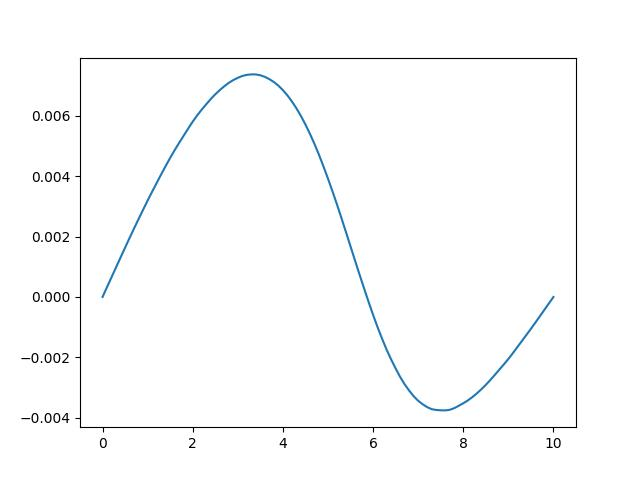
\includegraphics[width=1\linewidth]{2/z_V_3nst4_.jpg} 
		\caption{Изменение скорости на слое $3n_{st} / 4$}
	\end{minipage}
	\hfill
	\begin{minipage}[h]{0.47\linewidth}
		\centering
		\includegraphics[width=1\linewidth]{1/z_V_nst_.jpg} 
		\caption{Изменение скорости на слое $n_{st}$}
	\end{minipage}
	\caption{Графики изменения скорости для $\tau = 0.1, \ h = 0.1, \ C_{\rho} = 1, \ \mu = 0.1$}
	\label{ris:experimentalcorrelationsignals}
\end{figure}

\begin{figure}[h]
	\centering
	% Первая картинка
	\begin{minipage}[b]{0.49\linewidth}
		\centering
		\includegraphics[width=\textwidth]{1/z_H_e.jpg}  % Путь к первой картинке
		\caption{Изменение плотности}
	\end{minipage}%
	\hfill
	% Вторая картинка
	\begin{minipage}[b]{0.49\linewidth}
		\centering
		\includegraphics[width=\textwidth]{1/z_V_e.jpg}  % Путь ко второй картинке
		\caption{Изменение скорости}
	\end{minipage}
	\caption{Графики для $\tau = 0.1, \ h = 0.1, \ \gamma = 1.4, \ \mu = 0.1$}
	\label{ris:images}
\end{figure}

\begin{figure}[h]
	\begin{minipage}[h]{0.47\linewidth}
		\centering
		\includegraphics[width=1\linewidth]{1/z_H_nst4_e.jpg} 
		\caption{Изменение плотности на слое $n_{st} / 4$}
	\end{minipage}
	\hfill
	\begin{minipage}[h]{0.47\linewidth}
		\centering
		\includegraphics[width=1\linewidth]{1/z_H_nst2_e.jpg} 
		\caption{Изменение плотности на слое $n_{st} / 2$}
	\end{minipage}
\end{figure}
\begin{figure}[h]
	\begin{minipage}[h]{0.47\linewidth}
		\centering
		\includegraphics[width=1\linewidth]{1/z_H_3nst4_e.jpg} 
		\caption{Изменение плотности на слое $3n_{st} / 4$}
	\end{minipage}
	\hfill
	\begin{minipage}[h]{0.47\linewidth}
		\centering
		\includegraphics[width=1\linewidth]{1/z_H_nst_e.jpg} 
		\caption{Изменение плотности на слое $n_{st}$}
	\end{minipage}
	\caption{Графики изменения плотности для $\tau = 0.1, \ h = 0.1, \ \gamma = 1.4, \ \mu = 0.1$}
	\label{ris:experimentalcorrelationsignals}
\end{figure}

\begin{figure}[h]
	\begin{minipage}[h]{0.47\linewidth}
		\centering
		\includegraphics[width=1\linewidth]{1/z_V_nst4_e.jpg} 
		\caption{Изменение скорости на слое $n_{st} / 4$}
	\end{minipage}
	\hfill
	\begin{minipage}[h]{0.47\linewidth}
		\centering
		\includegraphics[width=1\linewidth]{1/z_V_nst2_e.jpg} 
		\caption{Изменение скорости на слое $n_{st} / 2$}
	\end{minipage}
	\vfill
	\begin{minipage}[h]{0.47\linewidth}
		\centering
		\includegraphics[width=1\linewidth]{1/z_V_3nst4_e.jpg} 
		\caption{Изменение скорости на слое $3n_{st} / 4$}
	\end{minipage}
	\hfill
	\begin{minipage}[h]{0.47\linewidth}
		\centering
		\includegraphics[width=1\linewidth]{1/z_V_nst_e.jpg} 
		\caption{Изменение скорости на слое $n_{st}$}
	\end{minipage}
	\caption{Графики изменения скорости для $\tau = 0.1, \ h = 0.1, \ \gamma = 1.4, \ \mu = 0.1$}
	\label{ris:experimentalcorrelationsignals}
\end{figure}

\clearpage
\newpage
Ниже приведены таблицы содержащие времена стабилизации $T_{st}$ решений второй системы и величин $|| (H^{n_{st}}, V^{n_{st}}) - (\tilde{H}, \tilde{V})||_{C_h}$ при различных входных параметрах (строки таблицы) на разных временных слоях (столбцы таблицы). Так же приведены таблицы, содержащие величины 
\begin{equation*}
	\displaystyle \Delta_m (n) = \frac{\sum\limits_{m \in \bar{\omega}_h} H^n_m - \sum\limits_{m \in \bar{\omega}_h} H^0_m}{\sum\limits_{m \in \bar{\omega}_h} H^0_m}
\end{equation*}
на разных временных слоях (столбцы таблицы) при различных входных параметрах (строки таблицы).
\subsubsection{Таблицы для второй системы}

1. $C_{\rho} = 1, \ \mu = 0.1$
\begin{center}
	\begin{tabular}{ |c|c|c|c|c|c| } 
		\hline
		$\tau$, h & $n_{st}/ 4$ & $n_{st}/ 2$ & $3n_{st}/ 4$ & $n_{st}$ & $T_{st}$ \\ 
		\hline
		1e-01, 1e-01 & 4.240e-03 & 7.926e-04 & 3.560e-04 & 4.980e-05 & 3252.0\\ 
		\hline
		1e-01, 1e-02 & 1.310e-02 & 7.075e-03 & 2.204e-03 & 9.584e-04 & 7230.2\\ 
		\hline
		1e-02, 1e-01 & 4.634e-03 & 3.106e-04 & 2.039e-05 & 9.994e-07 & 2295.54\\ 
		\hline
		1e-02, 1e-02 & 2.997e-02 & 9.378e-03 & 3.115e-03 & 9.982e-04 & 882.29\\ 
		\hline
	\end{tabular}
\end{center}

\begin{center}
	\begin{tabular}{ |c|c|c|c|c| } 
		\hline
		$\tau$, h & $\Delta_m (n_{st}/ 4)$ & $\Delta_m (n_{st}/ 2)$ & $\Delta_m (3n_{st}/ 4)$ & $\Delta_m (n_{st})$ \\ 
		\hline
		1e-01, 1e-01 & -3.188e-01 & -3.393e-01 & -3.432e-01 & -3.443e-01 \\ 
		\hline
		1e-01, 1e-02 & -1.515e-01 & -1.720e-01 & -2.209e-01 & -2.444e-01 \\ 
		\hline
		1e-02, 1e-01 & -9.427e-02 & -9.608e-02 & -9.620e-02 & -9.620e-02 \\ 
		\hline
		1e-02, 1e-02 & -8.733e-03 & -9.626e-03 & -9.917e-03 & -1.002e-02 \\ 
		\hline
	\end{tabular}
\end{center}

2. $C_{\rho} = 1, \ \mu = 0.01$
\begin{center}
	\begin{tabular}{ |c|c|c|c|c|c| } 
		\hline
		$\tau$, h & $n_{st}/ 4$ & $n_{st}/ 2$ & $3n_{st}/ 4$ & $n_{st}$ & $T_{st}$ \\ 
		\hline
		1e-02, 1e-01 & 2.420e-03 & 6.126e-05 & 2.775e-05 & 9.913e-07 & 4060.64\\ 
		\hline
		1e-02, 1e-02 & 5.016e-02 & 4.545e-02 & 2.405e-02 & 9.973e-03 & 691.75\\ 
		\hline
		1e-03, 1e-01 & 1.476e-02 & 3.562e-03 & 1.169e-03 & 1.999e-04 & 340.797\\ 
		\hline
		1e-03, 1e-02 & 1.348e-01 & 7.861e-02 & 8.904e-02 & 4.000e-02 & 147.892\\ 
		\hline
	\end{tabular}
\end{center}

\begin{center}
	\begin{tabular}{ |c|c|c|c|c| } 
		\hline
		$\tau$, h & $\Delta_m (n_{st}/ 4)$ & $\Delta_m (n_{st}/ 2)$ & $\Delta_m (3n_{st}/ 4)$ & $\Delta_m (n_{st})$ \\ 
		\hline
		1e-02, 1e-01 & -8.250e-01 & -8.255e-01 & -8.255e-01 & -8.256e-01 \\ 
		\hline
		1e-02, 1e-02 & -3.657e-01 & -3.758e-01 & -3.813e-01 & -3.840e-01 \\ 
		\hline
		1e-03, 1e-01 & -7.855e-01 & -7.927e-01 & -7.942e-01 & -7.947e-01 \\ 
		\hline
		1e-03, 1e-02 & -2.590e-02 & -5.641e-02 & -6.694e-02 & -7.169e-02 \\ 
		\hline
	\end{tabular}
\end{center}

3. $C_{\rho} = 1, \ \mu = 0.001$
\begin{center}
	\begin{tabular}{ |c|c|c|c|c|c| } 
		\hline
		$\tau$, h & $n_{st}/ 4$ & $n_{st}/ 2$ & $3n_{st}/ 4$ & $n_{st}$ & $T_{st}$ \\ 
		\hline
		1e-03, 1e-02 & 5.664e-02 & 3.272e-02 & 3.500e-02 & 9.999e-03 & 139.701\\ 
		\hline
		1e-04, 1e-02 & 6.939e-01 & 2.490e-01 & 1.204e-01 & 9.999e-02 & 17.5948\\ 
		\hline
		1e-04, 1e-03 & 2.482e-01 & 2.577e-01 & 1.324e-01 & 1.000e-01 & 57.4926\\ 
		\hline
		1e-04, 5e-03 & 4.866e-01 & 2.676e-01 & 7.889e-02 & 4.998e-02 & 21.5834\\ 
		\hline
	\end{tabular}
\end{center}

\begin{center}
	\begin{tabular}{ |c|c|c|c|c| } 
		\hline
		$\tau$, h & $\Delta_m (n_{st}/ 4)$ & $\Delta_m (n_{st}/ 2)$ & $\Delta_m (3n_{st}/ 4)$ & $\Delta_m (n_{st})$ \\ 
		\hline
		1e-03, 1e-02 & -8.179e-01 & -8.224e-01 & -8.238e-01 & -8.247e-01 \\ 
		\hline
		1e-04, 1e-02 & -4.119e-01 & -7.533e-01 & -7.759e-01 & -7.830e-01 \\ 
		\hline
		1e-04, 1e-03 & -2.018e-02 & -2.545e-02 & -3.370e-02 & -4.811e-02 \\ 
		\hline
		1e-04, 5e-03 & -4.506e-01 & -5.645e-01 & -5.845e-01 & -5.911e-01 \\ 
		\hline
	\end{tabular}
\end{center}

4. $C_{\rho} = 10, \ \mu = 0.1$
\begin{center}
	\begin{tabular}{ |c|c|c|c|c|c| } 
		\hline
		$\tau$, h & $n_{st}/ 4$ & $n_{st}/ 2$ & $3n_{st}/ 4$ & $n_{st}$ & $T_{st}$ \\ 
		\hline
		1e-02, 1e-01 & 1.717e-02 & 1.551e-02 & 2.266e-03 & 9.669e-05 & 294.1\\ 
		\hline
		1e-02, 1e-02 & 2.478e-01 & 1.978e-01 & 1.240e-01 & 4.969e-02 & 103.42\\ 
		\hline
		1e-03, 1e-01 & 1.225e-02 & 2.116e-02 & 8.215e-03 & 9.993e-04 & 426.676\\ 
		\hline
		1e-03, 1e-02 & 1.304e-01 & 5.164e-02 & 2.450e-02 & 9.996e-03 & 201.059\\ 
		\hline
	\end{tabular}
\end{center}

\begin{center}
	\begin{tabular}{ |c|c|c|c|c| } 
		\hline
		$\tau$, h & $\Delta_m (n_{st}/ 4)$ & $\Delta_m (n_{st}/ 2)$ & $\Delta_m (3n_{st}/ 4)$ & $\Delta_m (n_{st})$ \\ 
		\hline
		1e-02, 1e-01 & -5.727e-01 & -5.853e-01 & -5.886e-01 & -5.893e-01 \\ 
		\hline
		1e-02, 1e-02 & -1.299e-01 & -1.565e-01 & -1.701e-01 & -1.808e-01 \\ 
		\hline
		1e-03, 1e-01 & -3.722e-01 & -3.778e-01 & -3.805e-01 & -3.823e-01 \\ 
		\hline
		1e-03, 1e-02 & -4.720e-03 & -7.215e-03 & -8.229e-03 & -8.799e-03 \\ 
		\hline
	\end{tabular}
\end{center}

5. $C_{\rho} = 10, \ \mu = 0.01$
\begin{center}
	\begin{tabular}{ |c|c|c|c|c|c| } 
		\hline
		$\tau$, h & $n_{st}/ 4$ & $n_{st}/ 2$ & $3n_{st}/ 4$ & $n_{st}$ & $T_{st}$ \\ 
		\hline
		1e-02, 1e-01 & 4.589e-03 & 2.739e-04 & 1.559e-05 & 9.853e-11 & 3195.61\\ 
		\hline
		1e-03, 1e-01 & 8.293e-02 & 1.116e-02 & 4.091e-03 & 9.984e-04 & 239.415\\ 
		\hline
		1e-03, 1e-02 & 5.475e-02 & 2.402e-02 & 3.342e-02 & 9.995e-03 & 587.866\\ 
		\hline
		1e-03, 1e-03 & 2.966e-01 & 2.398e-01 & 1.548e-01 & 9.989e-02 & 24.231\\ 
		\hline
	\end{tabular}
\end{center}

\begin{center}
	\begin{tabular}{ |c|c|c|c|c| } 
		\hline
		$\tau$, h & $\Delta_m (n_{st}/ 4)$ & $\Delta_m (n_{st}/ 2)$ & $\Delta_m (3n_{st}/ 4)$ & $\Delta_m (n_{st})$ \\ 
		\hline
		1e-02, 1e-01 & -9.597e-01 & -9.598e-01 & -9.598e-01 & -9.598e-01 \\ 
		\hline
		1e-03, 1e-01 & -9.367e-01 & -9.378e-01 & -9.381e-01 & -9.381e-01 \\ 
		\hline
		1e-03, 1e-02 & -5.998e-01 & -6.013e-01 & -6.023e-01 & -6.032e-01 \\ 
		\hline
		1e-03, 1e-03 & -1.623e-01 & -1.799e-01 & -1.914e-01 & -2.007e-01 \\ 
		\hline
	\end{tabular}
\end{center}

6. $C_{\rho} = 10, \ \mu = 0.001$
\begin{center}
	\begin{tabular}{ |c|c|c|c|c|c| } 
		\hline
		$\tau$, h & $n_{st}/ 4$ & $n_{st}/ 2$ & $3n_{st}/ 4$ & $n_{st}$ & $T_{st}$ \\ 
		\hline
		1e-04, 1e-03 & 6.669e-01 & 2.933e-01 & 1.659e-01 & 9.989e-02 & 7.0227\\ 
		\hline
		1e-04, 1e-04 & 2.579e-01 & 1.760e-01 & 2.071e-01 & 9.990e-02 & 14.5659\\ 
		\hline
		1e-05, 1e-03 & 2.405e-01 & 1.236e-01 & 2.385e-01 & 9.995e-02 & 16.56307\\ 
		\hline
		1e-05, 1e-04 & 2.295e-01 & 1.683e-01 & 2.307e-01 & 9.936e-02 & 19.76507\\ 
		\hline
	\end{tabular}
\end{center}

\begin{center}
	\begin{tabular}{ |c|c|c|c|c| } 
		\hline
		$\tau$, h & $\Delta_m (n_{st}/ 4)$ & $\Delta_m (n_{st}/ 2)$ & $\Delta_m (3n_{st}/ 4)$ & $\Delta_m (n_{st})$ \\ 
		\hline
		1e-04, 1e-03 & -5.571e-01 & -5.926e-01 & -5.957e-01 & -5.972e-01 \\ 
		\hline
		1e-04, 1e-04 & -1.798e-01 & -2.108e-01 & -2.256e-01 & -2.343e-01 \\ 
		\hline
		1e-05, 1e-03 & -1.693e-01 & -2.403e-01 & -2.043e-01 & -1.939e-02 \\ 
		\hline
		1e-05, 1e-04 & -1.605e-01 & -1.466e-01 & -1.055e-01 & -1.909e-02 \\ 
		\hline
	\end{tabular}
\end{center}

7. $C_{\rho} = 100, \ \mu = 0.1$
\begin{center}
	\begin{tabular}{ |c|c|c|c|c|c| } 
		\hline
		$\tau$, h & $n_{st}/ 4$ & $n_{st}/ 2$ & $3n_{st}/ 4$ & $n_{st}$ & $T_{st}$ \\ 
		\hline
		1e-03, 1e-01 & 3.827e-02 & 7.681e-03 & 1.128e-03 & 9.777e-06 & 313.255\\ 
		\hline
		1e-04, 1e-01 & 6.820e-02 & 5.212e-02 & 2.006e-02 & 9.987e-04 & 115.2639\\ 
		\hline
		1e-03, 1e-02 & 1.705e-01 & 6.334e-02 & 4.986e-02 & 9.675e-03 & 137.214\\ 
		\hline
		1e-04, 1e-02 & 3.141e-01 & 2.386e-01 & 2.093e-01 & 9.994e-02 & 21.6863\\ 
		\hline
	\end{tabular}
\end{center}

\begin{center}
	\begin{tabular}{ |c|c|c|c|c| } 
		\hline
		$\tau$, h & $\Delta_m (n_{st}/ 4)$ & $\Delta_m (n_{st}/ 2)$ & $\Delta_m (3n_{st}/ 4)$ & $\Delta_m (n_{st})$ \\ 
		\hline
		1e-03, 1e-01 & -8.229e-01 & -8.242e-01 & -8.243e-01 & -8.244e-01 \\ 
		\hline
		1e-04, 1e-02 & -7.972e-01 & -7.980e-01 & -7.985e-01 & -7.988e-01 \\ 
		\hline
		1e-03, 1e-02 & -3.443e-01 & -3.494e-01 & -3.518e-01 & -3.572e-01 \\ 
		\hline
		1e-04, 1e-02 & -9.908e-04 & -1.712e-03 & -2.196e-03 & -2.684e-03 \\ 
		\hline
	\end{tabular}
\end{center}

8. $C_{\rho} = 100, \ \mu = 0.01$
\begin{center}
	\begin{tabular}{ |c|c|c|c|c|c| } 
		\hline
		$\tau$, h & $n_{st}/ 4$ & $n_{st}/ 2$ & $3n_{st}/ 4$ & $n_{st}$ & $T_{st}$ \\ 
		\hline
		1e-04, 1e-02 & 7.101e-01 & 4.201e-01 & 2.824e-01 & 1.000e-01 & 10.5744\\ 
		\hline
		1e-04, 1e-03 & 3.540e-01 & 2.302e-01 & 2.295e-01 & 9.967e-02 & 16.6095\\ 
		\hline
		1e-04, 1e-04 & 2.184e-01 & 1.949e-01 & 1.728e-01 & 9.954e-02 & 21.4930\\ 
		\hline
		1e-05, 1e-04 & 1.928e-01 & 1.749e-01 & 1.492e-01 & 9.902e-01 & 24.29384\\ 
		\hline
	\end{tabular}
\end{center}

\begin{center}
	\begin{tabular}{ |c|c|c|c|c| } 
		\hline
		$\tau$, h & $\Delta_m (n_{st}/ 4)$ & $\Delta_m (n_{st}/ 2)$ & $\Delta_m (3n_{st}/ 4)$ & $\Delta_m (n_{st})$ \\ 
		\hline
		1e-04, 1e-02 & -8.176e-01 & -8.225e-01 & -8.240e-01 & -8.247e-01 \\ 
		\hline
		1e-04, 1e-03 & -3.410e-01 & -3.484e-01 & -3.517e-01 & -3.535e-01 \\ 
		\hline
		1e-04, 1e-04 & -1.395e-01 & -2.403e-01 & -2.103e-01 & -1.249e-01 \\ 
		\hline
		1e-05, 1e-05 & -1.234e-01 & -1.339e-01 & -1.293e-01 & -1.111e-01 \\ 
		\hline
	\end{tabular}
\end{center}

9. $C_{\rho} = 100, \ \mu = 0.001$
\begin{center}
	\begin{tabular}{ |c|c|c|c|c|c| } 
		\hline
		$\tau$, h & $n_{st}/ 4$ & $n_{st}/ 2$ & $3n_{st}/ 4$ & $n_{st}$ & $T_{st}$ \\ 
		\hline
		1e-04, 1e-04 & 2.585e-01 & 1.255e-01 & 2.485e-01 & 9.245e-02 & 9.3575\\ 
		\hline
		1e-04, 1e-05 & 2.469e-01 & 1.757e-01 & 2.477e-01 & 9.945e-02 & 11.7436\\ 
		\hline
		1e-05, 1e-04 & 2.445e-01 & 1.256e-01 & 2.585e-01 & 9.995e-02 & 13.55678\\ 
		\hline
		1e-05, 1e-05 & 2.485e-01 & 2.3943e-01 & 1.049e-01 & 9.999e-02 & 20.54838\\ 
		\hline
	\end{tabular}
\end{center}

\begin{center}
	\begin{tabular}{ |c|c|c|c|c| } 
		\hline
		$\tau$, h & $\Delta_m (n_{st}/ 4)$ & $\Delta_m (n_{st}/ 2)$ & $\Delta_m (3n_{st}/ 4)$ & $\Delta_m (n_{st})$ \\ 
		\hline
		1e-04, 1e-04 & -1.394e-01 & -2.294e-01 & -2.294e-01 & -2.-295e-01 \\ 
		\hline
		1e-04, 1e-05 & -2.842e-01 & -1.283e-01 & -1.392e-01 & -1.384e-01 \\ 
		\hline
		1e-05, 1e-04 & -3.293-01 & -1.239e-01 & -1.395-01 & -8.294e-02 \\ 
		\hline
		1e-05, 1e-05 & -1.293e-01 & -1.120e-01 & -9.938e-02 & -9.834e-02 \\ 
		\hline
	\end{tabular}
\end{center}

10. $\gamma = 1.4, \ \mu = 0.1$
\begin{center}
	\begin{tabular}{ |c|c|c|c|c|c| } 
		\hline
		$\tau$, h & $n_{st}/ 4$ & $n_{st}/ 2$ & $3n_{st}/ 4$ & $n_{st}$ & $T_{st}$ \\ 
		\hline
		1e-01, 1e-01 & 4.558e-03 & 1.155e-03 & 7.850e-05 & 4.997e-05 & 2418.5\\ 
		\hline
		1e-01, 1e-02 & 1.670e-02 & 5.063e-03 & 2.587e-03 & 9.932e-04 & 1506.2\\ 
		\hline
		1e-02, 1e-01 & 2.175e-02 & 1.043e-02 & 2.862e-03 & 9.981e-04 & 816.63\\ 
		\hline
		1e-02, 1e-02 & 2.389e-02 & 7.778e-03 & 3.787e-03 & 9.966e-04 & 857.32\\ 
		\hline
	\end{tabular}
\end{center}

\begin{center}
	\begin{tabular}{ |c|c|c|c|c| } 
		\hline
		$\tau$, h & $\Delta_m (n_{st}/ 4)$ & $\Delta_m (n_{st}/ 2)$ & $\Delta_m (3n_{st}/ 4)$ & $\Delta_m (n_{st})$ \\ 
		\hline
		1e-01, 1e-01 & -4.140e-01 & -4.161e-01 & -4.171e-01 & -4.174e-01 \\ 
		\hline
		1e-01, 1e-02 & -3.476e-01 & -3.485e-01 & -3.488e-01 & -3.497e-01 \\ 
		\hline
		1e-02, 1e-01 & -9.636e-02 & -1.042e-01 & -1.067e-01 & -1.077e-01 \\ 
		\hline
		1e-02, 1e-02 & -9.308e-03 & -1.011e-02 & -1.038e-02 & -1.049e-02 \\ 
		\hline
	\end{tabular}
\end{center}

11. $\gamma = 1.4, \ \mu = 0.01$
\begin{center}
	\begin{tabular}{ |c|c|c|c|c|c| } 
		\hline
		$\tau$, h & $n_{st}/ 4$ & $n_{st}/ 2$ & $3n_{st}/ 4$ & $n_{st}$ & $T_{st}$ \\ 
		\hline
		1e-02, 1e-01 & 1.161e-02 & 1.348e-03 & 1.155e-03 & 9.970e-05 & 2531.09\\ 
		\hline
		1e-01, 1e-02 & 8.478e-03 & 3.473e-03 & 1.612e-03 & 9.908e-05 & 2396.1\\ 
		\hline
		1e-02, 1e-02 & 2.500e-02 & 2.242e-02 & 1.536e-02 & 9.997e-03 & 610.05\\ 
		\hline
		1e-03. 1e-01 & 6.304e-02 & 4.850e-02 & 2.548e-02 & 9.998e-03 & 358.151\\ 
		\hline
	\end{tabular}
\end{center}

\begin{center}
	\begin{tabular}{ |c|c|c|c|c| } 
		\hline
		$\tau$, h & $\Delta_m (n_{st}/ 4)$ & $\Delta_m (n_{st}/ 2)$ & $\Delta_m (3n_{st}/ 4)$ & $\Delta_m (n_{st})$ \\ 
		\hline
		1e-02, 1e-01 & -7.940e-01 & -7.962e-01 & -7.968e-01 & -7.970e-01 \\ 
		\hline
		1e-01, 1e-02 & -8.893e-01 & -8.895e-01 & -8.895e-01 & -8.895e-01 \\ 
		\hline
		1e-02, 1e-02 & -4.454e-01 & -4.491e-01 & -4.529e-01 & -4.550e-01 \\ 
		\hline
		1e-03, 1e-01 & -7.528e-01 & -7.597e-01 & -7.651e-01 & -7.679e-01 \\ 
		\hline
	\end{tabular}
\end{center}

12. $\gamma = 1.4, \ \mu = 0.001$
\begin{center}
	\begin{tabular}{ |c|c|c|c|c|c| } 
		\hline
		$\tau$, h & $n_{st}/ 4$ & $n_{st}/ 2$ & $3n_{st}/ 4$ & $n_{st}$ & $T_{st}$ \\ 
		\hline
		1e-03, 1e-02 & 5.632e-02 & 3.318e-02 & 2.946e-02 & 9.997e-03 & 150.266\\ 
		\hline
		1e-04, 1e-02 & 5.659e-01 & 3.775e-01 & 2.741e-01 & 9.999e-02 & 14.8061\\ 
		\hline
		1e-03, 1e-03 & 4.057e-01 & 2.019e-01 & 1.823e-01 & 9.993e-02 & 15.979\\ 
		\hline
		1e-02, 1e-03 & 8.980e-01 & 2.083e-01 & 2.025e-01 & 9.992e-02 & 46.83\\ 
		\hline
	\end{tabular}
\end{center}

\begin{center}
	\begin{tabular}{ |c|c|c|c|c| } 
		\hline
		$\tau$, h & $\Delta_m (n_{st}/ 4)$ & $\Delta_m (n_{st}/ 2)$ & $\Delta_m (3n_{st}/ 4)$ & $\Delta_m (n_{st})$ \\ 
		\hline
		1e-03, 1e-02 & -7.891e-01 & -7.921e-01 & -7.934e-01 & -7.941e-01 \\ 
		\hline
		1e-04, 1e-02 & -4.030e-01 & -7.212e-01 & -7.379e-01 & -7.591e-01 \\ 
		\hline
		1e-03, 1e-03 & -3.617e-01 & -4.172e-01 & -4.210e-01 & -4.239e-01 \\ 
		\hline
		1e-02, 1e-03 & -8.741e-01 & -8.791e-01 & -8.803e-01 & -8.809e-01 \\ 
		\hline
	\end{tabular}
\end{center}

\subsubsection{Графики для второй системы}

\begin{figure}[h]
	\centering
	% Первая картинка
	\begin{minipage}[b]{0.49\linewidth}
		\centering
		\includegraphics[width=\textwidth]{2/z_H_.jpg}  % Путь к первой картинке
		\caption{Изменение плотности}
	\end{minipage}%
	\hfill
	% Вторая картинка
	\begin{minipage}[b]{0.49\linewidth}
		\centering
		\includegraphics[width=\textwidth]{2/z_V_.jpg}  % Путь ко второй картинке
		\caption{Изменение скорости}
	\end{minipage}
	\caption{Графики для $\tau = 0.1, \ h = 0.1, \ C_{\rho} = 1, \ \mu = 0.1$}
	\label{ris:images}
\end{figure}

\begin{figure}[h]
	\begin{minipage}[h]{0.47\linewidth}
		\centering
		\includegraphics[width=1\linewidth]{2/z_H_nst4_.jpg} 
		\caption{Изменение плотности на слое $n_{st} / 4$}
	\end{minipage}
	\hfill
	\begin{minipage}[h]{0.47\linewidth}
		\centering
		\includegraphics[width=1\linewidth]{2/z_H_nst2_.jpg} 
		\caption{Изменение плотности на слое $n_{st} / 2$}
	\end{minipage}
\end{figure}
\begin{figure}[h]
	\begin{minipage}[h]{0.47\linewidth}
		\centering
		\includegraphics[width=1\linewidth]{2/z_H_3nst4_.jpg} 
		\caption{Изменение плотности на слое $3n_{st} / 4$}
	\end{minipage}
	\hfill
	\begin{minipage}[h]{0.47\linewidth}
		\centering
		\includegraphics[width=1\linewidth]{2/z_H_nst_.jpg} 
		\caption{Изменение плотности на слое $n_{st}$}
	\end{minipage}
	\caption{Графики изменения плотности для $\tau = 0.1, \ h = 0.1, \ C_{\rho} = 1, \ \mu = 0.1$}
	\label{ris:experimentalcorrelationsignals}
\end{figure}

\begin{figure}[h]
	\begin{minipage}[h]{0.47\linewidth}
		\centering
		\includegraphics[width=1\linewidth]{2/z_V_nst4_.jpg} 
		\caption{Изменение скорости на слое $n_{st} / 4$}
	\end{minipage}
	\hfill
	\begin{minipage}[h]{0.47\linewidth}
		\centering
		\includegraphics[width=1\linewidth]{2/z_V_nst2_.jpg} 
		\caption{Изменение скорости на слое $n_{st} / 2$}
	\end{minipage}
	\vfill
	\begin{minipage}[h]{0.47\linewidth}
		\centering
		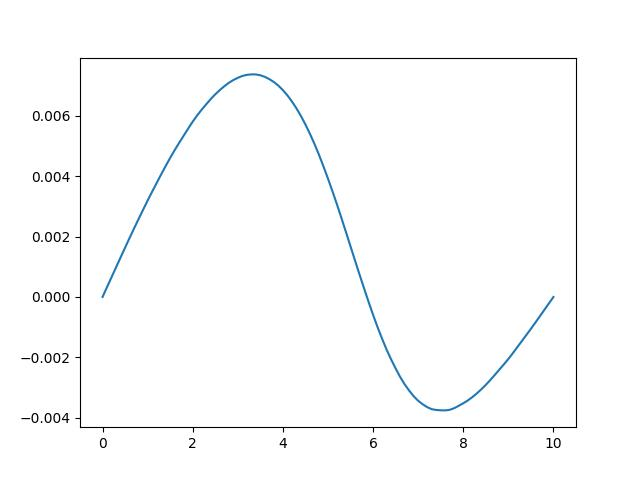
\includegraphics[width=1\linewidth]{2/z_V_3nst4_.jpg} 
		\caption{Изменение скорости на слое $3n_{st} / 4$}
	\end{minipage}
	\hfill
	\begin{minipage}[h]{0.47\linewidth}
		\centering
		\includegraphics[width=1\linewidth]{2/z_V_nst_.jpg} 
		\caption{Изменение скорости на слое $n_{st}$}
	\end{minipage}
	\caption{Графики изменения скорости для $\tau = 0.1, \ h = 0.1, \ C_{\rho} = 1, \ \mu = 0.1$}
	\label{ris:experimentalcorrelationsignals}
\end{figure}

\begin{figure}[h]
	\centering
	% Первая картинка
	\begin{minipage}[b]{0.49\linewidth}
		\centering
		\includegraphics[width=\textwidth]{2/z_H_e.jpg}  % Путь к первой картинке
		\caption{Изменение плотности}
	\end{minipage}%
	\hfill
	% Вторая картинка
	\begin{minipage}[b]{0.49\linewidth}
		\centering
		\includegraphics[width=\textwidth]{2/z_V_e.jpg}  % Путь ко второй картинке
		\caption{Изменение скорости}
	\end{minipage}
	\caption{Графики для $\tau = 0.1, \ h = 0.1, \ \gamma = 1.4, \ \mu = 0.1$}
	\label{ris:images}
\end{figure}

\begin{figure}[h]
	\begin{minipage}[h]{0.47\linewidth}
		\centering
		\includegraphics[width=1\linewidth]{2/z_H_nst4_e.jpg} 
		\caption{Изменение плотности на слое $n_{st} / 4$}
	\end{minipage}
	\hfill
	\begin{minipage}[h]{0.47\linewidth}
		\centering
		\includegraphics[width=1\linewidth]{2/z_H_nst2_e.jpg} 
		\caption{Изменение плотности на слое $n_{st} / 2$}
	\end{minipage}
	\vfill
	\begin{minipage}[h]{0.47\linewidth}
		\centering
		\includegraphics[width=1\linewidth]{2/z_H_3nst4_e.jpg} 
		\caption{Изменение плотности на слое $3n_{st} / 4$}
	\end{minipage}
	\hfill
	\begin{minipage}[h]{0.47\linewidth}
		\centering
		\includegraphics[width=1\linewidth]{2/z_H_nst_e.jpg} 
		\caption{Изменение плотности на слое $n_{st}$}
	\end{minipage}
	\caption{Графики изменения плотности для $\tau = 0.1, \ h = 0.1, \ \gamma = 1.4, \ \mu = 0.1$}
	\label{ris:experimentalcorrelationsignals}
\end{figure}

\begin{figure}[h]
	\begin{minipage}[h]{0.47\linewidth}
		\centering
		\includegraphics[width=1\linewidth]{2/z_V_nst4_e.jpg} 
		\caption{Изменение скорости на слое $n_{st} / 4$}
	\end{minipage}
	\hfill
	\begin{minipage}[h]{0.47\linewidth}
		\centering
		\includegraphics[width=1\linewidth]{2/z_V_nst2_e.jpg} 
		\caption{Изменение скорости на слое $n_{st} / 2$}
	\end{minipage}
	\vfill
	\begin{minipage}[h]{0.47\linewidth}
		\centering
		\includegraphics[width=1\linewidth]{2/z_V_3nst4_e.jpg} 
		\caption{Изменение скорости на слое $3n_{st} / 4$}
	\end{minipage}
	\hfill
	\begin{minipage}[h]{0.47\linewidth}
		\centering
		\includegraphics[width=1\linewidth]{2/z_V_nst_e.jpg} 
		\caption{Изменение скорости на слое $n_{st}$}
	\end{minipage}
	\caption{Графики изменения скорости для $\tau = 0.1, \ h = 0.1, \ \gamma = 1.4, \ \mu = 0.1$}
	\label{ris:experimentalcorrelationsignals}
\end{figure}